% COMP1551 Application Development - Coursework, Term 2 2025/26
% Tasks 1 and 2: system description, software requirements specification and
% the two UML diagrams. Task 3 is submitted separately as EducationCentreSystem.cs.
%
% Build: pdflatex COMP1551_report.tex   (run twice so the diagrams settle)

\documentclass[11pt,a4paper]{article}

\usepackage[margin=2.5cm]{geometry}
\usepackage[T1]{fontenc}
\usepackage{tgpagella}
\usepackage[sc]{mathpazo}
\usepackage{courier}
\usepackage{microtype}
\linespread{1.05}

\usepackage{tikz}
\usetikzlibrary{positioning,shapes.multipart,shapes.geometric,arrows,calc,fit}
\usepackage{float}
\usepackage{caption}
\usepackage{xcolor}
\usepackage{titlesec}
\usepackage{hyperref}
\usepackage{xurl}   % lets the long GitHub address break across lines

\hypersetup{
  colorlinks = true,
  urlcolor   = [HTML]{1A5FB4},
  linkcolor  = black,
  breaklinks = true,
  pdfauthor  = {Phan The Viet},
  pdftitle   = {COMP1551 Coursework: Education Centre Desktop Information System},
  pdfsubject = {Tasks 1 and 2},
}

\captionsetup{font=small,labelfont=bf}
\titlespacing*{\section}{0pt}{1.1em}{0.5em}
\titlespacing*{\subsection}{0pt}{0.9em}{0.3em}
\setlength{\parskip}{0.35em}
\setlength{\parindent}{0pt}

% ---------------------------------------------------------------------------
% Diagram styles
% ---------------------------------------------------------------------------
\tikzset{
  umlclass/.style = {
    rectangle split, rectangle split parts=3, draw, thick,
    text width=#1, align=left, font=\scriptsize,
    inner sep=4pt, rectangle split part align=left
  },
  umlclass/.default = 4.6cm,
  umlbox/.style = {
    rectangle split, rectangle split parts=2, draw, thick,
    text width=#1, align=left, font=\scriptsize,
    inner sep=4pt, rectangle split part align=left
  },
  umlbox/.default = 4.6cm,
  inherit/.style  = {-open triangle 45, thick},
  compose/.style  = {diamond-, thick},
  assoc/.style    = {thick},
  depend/.style   = {-latex, thick, dashed},
  mult/.style     = {font=\scriptsize, inner sep=1.5pt},
  usecase/.style  = {ellipse, draw, thick, align=center, font=\scriptsize,
                     minimum width=3.1cm, minimum height=1.0cm, inner sep=2pt},
  stereo/.style   = {font=\scriptsize\itshape}
}

% A stick figure actor, drawn once and reused.
\newcommand{\actor}[3]{%
  \begin{scope}[shift={(#1)}]
    \draw[thick] (0,0.62) circle (0.17);
    \draw[thick] (0,0.45) -- (0,-0.05);
    \draw[thick] (-0.28,0.28) -- (0.28,0.28);
    \draw[thick] (0,-0.05) -- (-0.22,-0.5);
    \draw[thick] (0,-0.05) -- (0.22,-0.5);
    \node[font=\scriptsize, align=center] at (0,-0.85) {#2};
    \coordinate (#3) at (0.32,0.2);
  \end{scope}}

\begin{document}

% ---------------------------------------------------------------------------
% Title
% ---------------------------------------------------------------------------
\begin{center}
  {\large\textbf{COMP1551 Application Development}}\\[0.35em]
  {\Large\textbf{Education Centre Desktop Information System}}\\[0.6em]
  {\normalsize Coursework, Term 2 2025/26 --- Tasks 1 and 2}\\[1.0em]
  \begin{tabular}{rl}
    Student name & Phan The Viet\\
    Student ID   & GCS240020\\
    Module leader & Tuan Nguyen\\
  \end{tabular}
\end{center}

\vspace{0.4em}
\hrule
\vspace{0.8em}

Task 3 of this coursework is submitted separately as the single source file
\texttt{EducationCentre\allowbreak System.cs}. The two diagrams in Task 2
describe the classes and the behaviour of that file. The same file is published
at\\
{\small\url{https://github.com/ryanthemechanic/GRE-Coursework/blob/main/Year-2/Semester-2/COMP1551/EducationCentreSystem.cs}}

% ===========================================================================
\section*{Task 1a --- Description of the Desktop Information System}
\addcontentsline{toc}{section}{Task 1a}

\textit{275 words.}

The education centre keeps its records on paper. Teaching staff, administration
staff and students each have a folder of forms, and the office copies a form by
hand whenever somebody changes a telephone number or takes on a new subject.
Finding one record means going through a drawer, and the same person often
appears twice with different details.

For every person on the books the system holds a name, a telephone number, an
email address and the role that person has at the centre. Each group then has
details of its own. A member of the teaching staff has a salary and the two
subjects they teach. A member of the administration staff has a salary, the
hours worked each week, and whether the post is full time or part time. A
student has the three subjects they study.

The office needs five things from the program: add a new person to the records;
show every record held; show only the records of one group, so that the teaching
staff can be listed without the students in the way; change the details of a
person already recorded; and remove a person who has left the centre.

The program is for one member of the office staff at one machine. It should run
on the centre's existing Windows 10 or Windows 11 desktops, which have 8~GB of
memory and no graphics card beyond the one in the processor, and it should
install without database software or a network connection. The office would
rather type than use a mouse, so a numbered menu worked from the keyboard suits
the way the staff already work.

% ===========================================================================
\section*{Task 1b --- Software Requirements Specification}
\addcontentsline{toc}{section}{Task 1b}

\textit{378 words, excluding headings.}

{\footnotesize The structure and wording below follow Wiegers, K. and Beatty, J.
(2013) \textit{Software Requirements}. 3rd edn. Redmond, WA: Microsoft Press,
chapters 10 and 11.}

\subsection*{1. Introduction}

\textbf{Purpose.} This document specifies the Education Centre Desktop
Information System (ECDIS), version 1.0, which replaces the centre's paper
records.

\textbf{Project scope.} ECDIS records the teaching staff, administration staff
and students of one centre, and supports adding, viewing, filtering, editing and
deleting those records. Timetabling, payroll and marks are out of scope.

\subsection*{2. Overall Description}

\textbf{Product.} A self-contained desktop application. It connects to no other
system and holds its records in memory while it is running.

\textbf{Users.} One records officer in the centre office, familiar with Windows
but not with computing.

\textbf{Operational environment.} A Windows 10 or Windows 11 desktop with the
.NET runtime, 4~GB of memory, no network and no database server.

\subsection*{3. System Features}

\textbf{Description.} One record per person. Every record holds a name,
telephone number, email address and role; teaching staff records add a salary
and two subjects, administration records a salary, contract type and weekly
hours, and student records three subjects.

\textbf{Functional requirements.}
\begin{itemize}\setlength{\itemsep}{0pt}
  \item FR-1 The system shall present a menu of its operations and return to it
        when an operation ends.
  \item FR-2 The system shall add a record to one of the three groups, asking
        only for the fields that group holds.
  \item FR-3 The system shall refuse an empty or malformed name, telephone
        number, email address, salary or subject, and ask again.
  \item FR-4 The system shall list every record held with the fields belonging
        to it.
  \item FR-5 The system shall list the records of one group on request.
  \item FR-6 The system shall change any field of a chosen record, keeping the
        stored value where none is given.
  \item FR-7 The system shall delete a chosen record, after the user confirms.
  \item FR-8 The system shall store records in a structure whose size is not
        fixed in advance.
\end{itemize}

\subsection*{4. User Interface Requirements}

A keyboard-driven text interface. Menu options are numbered, prompts name the
field asked for, and while a record is edited its stored value is shown in
brackets.

\subsection*{5. Platform Requirements}

Windows 10 or Windows 11, 64-bit, with the .NET runtime. One executable, no
installer, and nothing written to disk.

\subsection*{6. Quality Attributes}

\textbf{Performance.} Any operation completes within one second for up to 1,000
records.

\textbf{Security.} The records are protected by the Windows account of the
single office machine.

\textbf{Safety.} Deletion is confirmed and invalid data refused at entry, so a
mistyped answer cannot corrupt the records.

% ===========================================================================
\clearpage
\section*{Task 2a --- UML Class Diagram}
\addcontentsline{toc}{section}{Task 2a}

Figure~\ref{fig:class} shows the classes of the system. \texttt{Person} is
abstract and holds the data every record has; \texttt{Teacher}, \texttt{Admin}
and \texttt{Student} inherit from it and add the fields of their own group,
overriding \texttt{Role}, \texttt{PrintDetails} and \texttt{CaptureDetails}.
\texttt{PersonRegister} owns the list that holds every record.
\texttt{Validation} and \texttt{Prompt} are static classes: the first states the
rule each field must satisfy, the second asks the questions at the keyboard and
repeats them until the rule is met. Private members are marked $-$, protected
members $\#$ and public members $+$.

\begin{figure}[H]
\centering
\resizebox{\textwidth}{!}{%
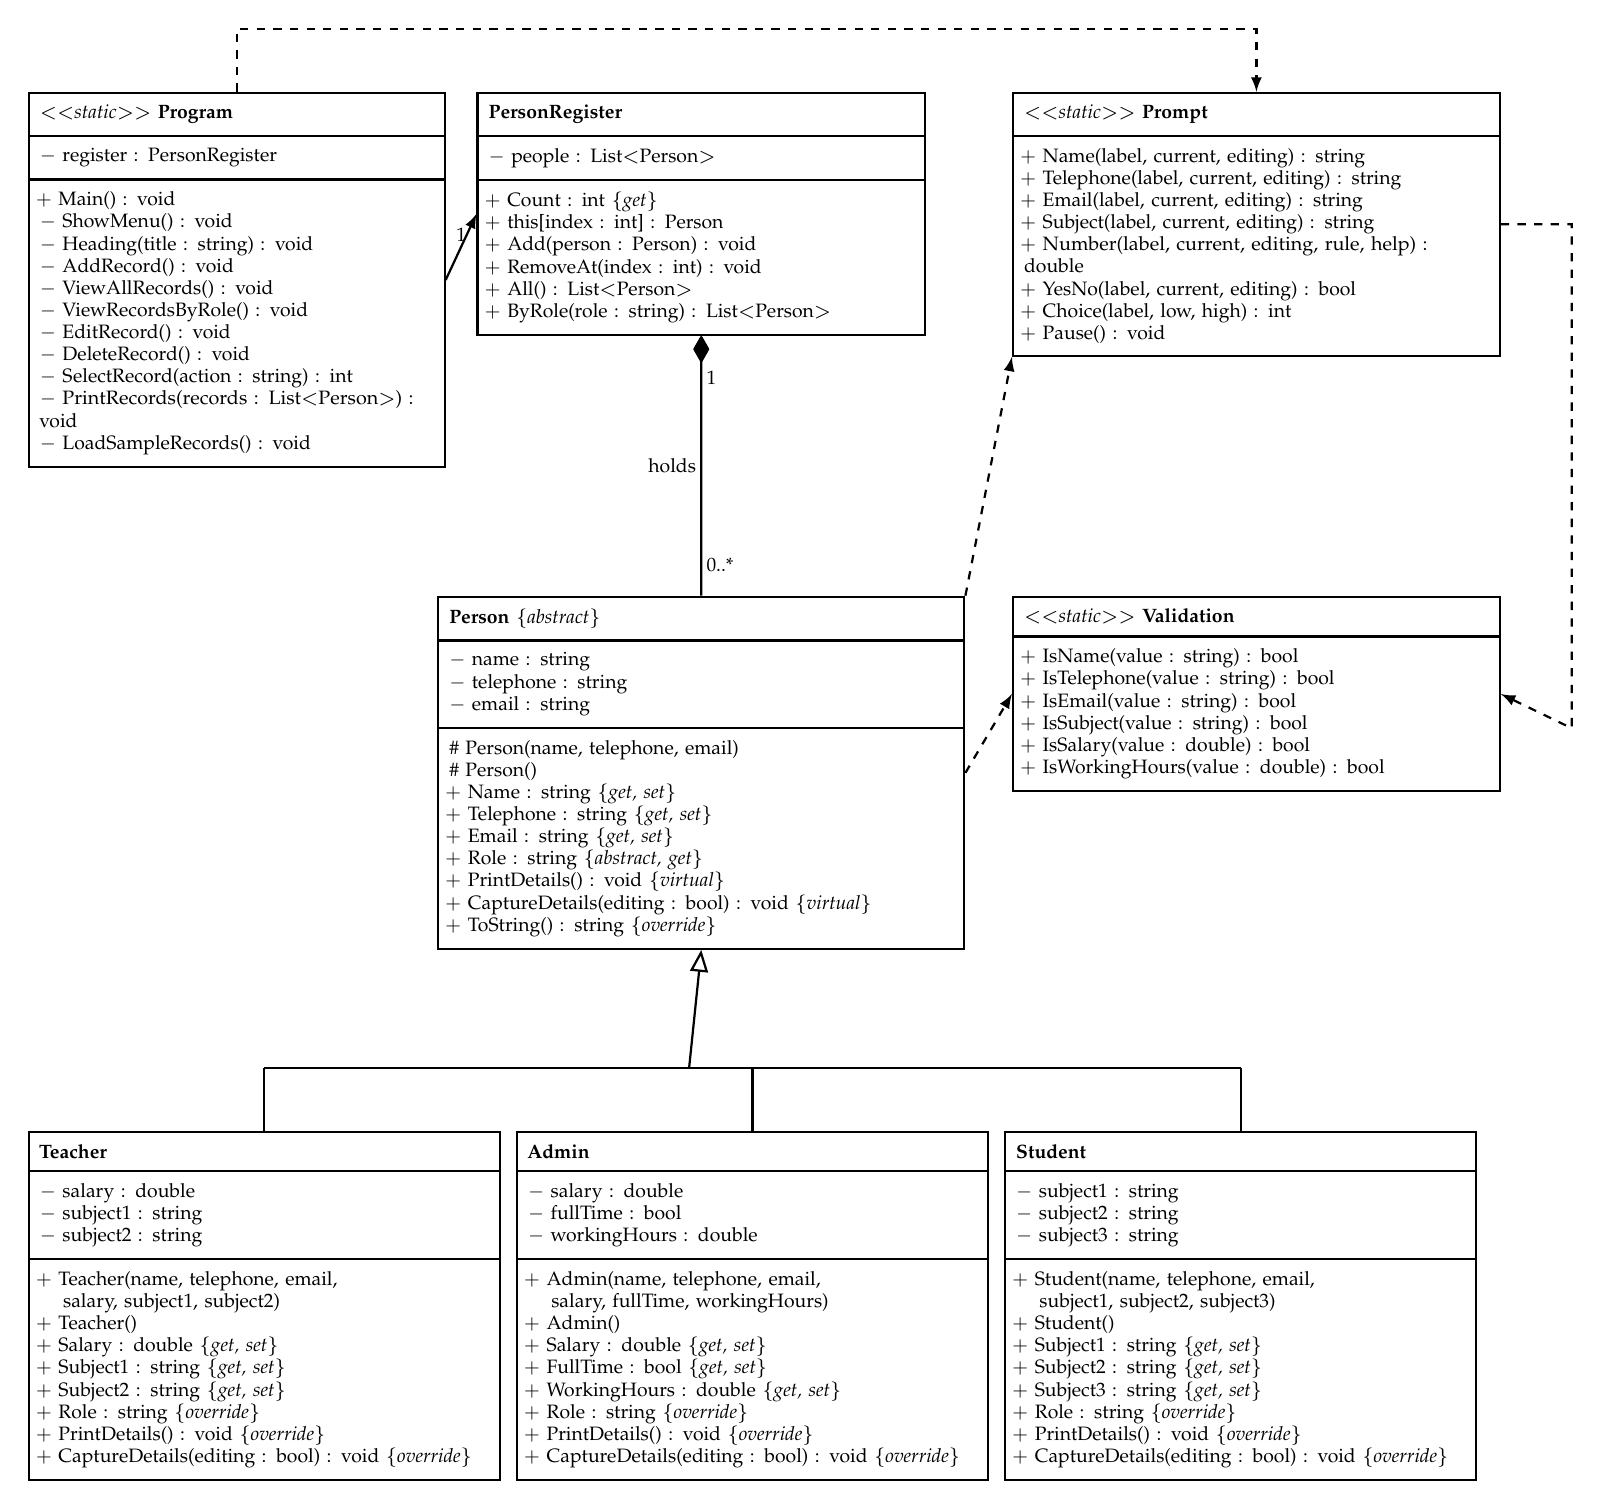
\begin{tikzpicture}[x=1cm,y=1cm]
\hyphenpenalty=10000 \exhyphenpenalty=10000  % no hyphens inside the boxes

% Every box is placed by its top-left corner on a fixed grid, so that nothing
% can drift into anything else when the drawing is scaled to the page width.

% --- row 1: the application, the store of records, and the input helper ----
\node[umlclass=5.0cm, anchor=north west] (program) at (0,0) {
  \textit{\textless\textless static\textgreater\textgreater}\ \textbf{Program}
  \nodepart{second}
  $-$ register : PersonRegister
  \nodepart{third}
  $+$ Main() : void\\
  $-$ ShowMenu() : void\\
  $-$ Heading(title : string) : void\\
  $-$ AddRecord() : void\\
  $-$ ViewAllRecords() : void\\
  $-$ ViewRecordsByRole() : void\\
  $-$ EditRecord() : void\\
  $-$ DeleteRecord() : void\\
  $-$ SelectRecord(action : string) : int\\
  $-$ PrintRecords(records : List\textless Person\textgreater) : void\\
  $-$ LoadSampleRecords() : void
};

\node[umlclass=5.4cm, anchor=north west] (register) at (5.7,0) {
  \textbf{PersonRegister}
  \nodepart{second}
  $-$ people : List\textless Person\textgreater
  \nodepart{third}
  $+$ Count : int \textit{\{get\}}\\
  $+$ this[index : int] : Person\\
  $+$ Add(person : Person) : void\\
  $+$ RemoveAt(index : int) : void\\
  $+$ All() : List\textless Person\textgreater\\
  $+$ ByRole(role : string) : List\textless Person\textgreater
};

\node[umlbox=5.9cm, anchor=north west] (prompt) at (12.5,0) {
  \textit{\textless\textless static\textgreater\textgreater}\ \textbf{Prompt}
  \nodepart{second}
  $+$ Name(label, current, editing) : string\\
  $+$ Telephone(label, current, editing) : string\\
  $+$ Email(label, current, editing) : string\\
  $+$ Subject(label, current, editing) : string\\
  $+$ Number(label, current, editing, rule, help) : double\\
  $+$ YesNo(label, current, editing) : bool\\
  $+$ Choice(label, low, high) : int\\
  $+$ Pause() : void
};

% --- row 2: the base class and the field rules ----------------------------
\node[umlclass=6.4cm, anchor=north west] (person) at (5.2,-6.4) {
  \textbf{Person} \textit{\{abstract\}}
  \nodepart{second}
  $-$ name : string\\
  $-$ telephone : string\\
  $-$ email : string
  \nodepart{third}
  $\#$ Person(name, telephone, email)\\
  $\#$ Person()\\
  $+$ Name : string \textit{\{get, set\}}\\
  $+$ Telephone : string \textit{\{get, set\}}\\
  $+$ Email : string \textit{\{get, set\}}\\
  $+$ Role : string \textit{\{abstract, get\}}\\
  $+$ PrintDetails() : void \textit{\{virtual\}}\\
  $+$ CaptureDetails(editing : bool) : void \textit{\{virtual\}}\\
  $+$ ToString() : string \textit{\{override\}}
};

\node[umlbox=5.9cm, anchor=north west] (validation) at (12.5,-6.4) {
  \textit{\textless\textless static\textgreater\textgreater}\ \textbf{Validation}
  \nodepart{second}
  $+$ IsName(value : string) : bool\\
  $+$ IsTelephone(value : string) : bool\\
  $+$ IsEmail(value : string) : bool\\
  $+$ IsSubject(value : string) : bool\\
  $+$ IsSalary(value : double) : bool\\
  $+$ IsWorkingHours(value : double) : bool
};

% --- row 3: the three derived classes -------------------------------------
\node[umlclass=5.7cm, anchor=north west] (teacher) at (0,-13.2) {
  \textbf{Teacher}
  \nodepart{second}
  $-$ salary : double\\
  $-$ subject1 : string\\
  $-$ subject2 : string
  \nodepart{third}
  $+$ Teacher(name, telephone, email,\\
  \hspace*{1.2em}salary, subject1, subject2)\\
  $+$ Teacher()\\
  $+$ Salary : double \textit{\{get, set\}}\\
  $+$ Subject1 : string \textit{\{get, set\}}\\
  $+$ Subject2 : string \textit{\{get, set\}}\\
  $+$ Role : string \textit{\{override\}}\\
  $+$ PrintDetails() : void \textit{\{override\}}\\
  $+$ CaptureDetails(editing : bool) : void \textit{\{override\}}
};

\node[umlclass=5.7cm, anchor=north west] (admin) at (6.2,-13.2) {
  \textbf{Admin}
  \nodepart{second}
  $-$ salary : double\\
  $-$ fullTime : bool\\
  $-$ workingHours : double
  \nodepart{third}
  $+$ Admin(name, telephone, email,\\
  \hspace*{1.2em}salary, fullTime, workingHours)\\
  $+$ Admin()\\
  $+$ Salary : double \textit{\{get, set\}}\\
  $+$ FullTime : bool \textit{\{get, set\}}\\
  $+$ WorkingHours : double \textit{\{get, set\}}\\
  $+$ Role : string \textit{\{override\}}\\
  $+$ PrintDetails() : void \textit{\{override\}}\\
  $+$ CaptureDetails(editing : bool) : void \textit{\{override\}}
};

\node[umlclass=5.7cm, anchor=north west] (student) at (12.4,-13.2) {
  \textbf{Student}
  \nodepart{second}
  $-$ subject1 : string\\
  $-$ subject2 : string\\
  $-$ subject3 : string
  \nodepart{third}
  $+$ Student(name, telephone, email,\\
  \hspace*{1.2em}subject1, subject2, subject3)\\
  $+$ Student()\\
  $+$ Subject1 : string \textit{\{get, set\}}\\
  $+$ Subject2 : string \textit{\{get, set\}}\\
  $+$ Subject3 : string \textit{\{get, set\}}\\
  $+$ Role : string \textit{\{override\}}\\
  $+$ PrintDetails() : void \textit{\{override\}}\\
  $+$ CaptureDetails(editing : bool) : void \textit{\{override\}}
};

% --- generalisation: the three subclasses share one triangle into Person ---
\coordinate (bus) at (8.4,-12.4);
\draw[assoc] (teacher.north) -- (teacher.north |- bus);
\draw[assoc] (admin.north)   -- (admin.north   |- bus);
\draw[assoc] (student.north) -- (student.north |- bus);
\draw[assoc] (teacher.north |- bus) -- (student.north |- bus);
\draw[inherit] (bus) -- (person.south);

% --- the register is composed of the records it holds ---------------------
\draw[compose] (register.south) -- node[mult, right, pos=0.16] {1}
                                   node[mult, right, pos=0.88] {0..*}
                                   node[mult, left, midway] {holds} (person.north);

% --- who uses whom --------------------------------------------------------
\draw[assoc, -latex] (program.east) -- node[mult, above, midway] {1} (register.west);
\draw[depend] (person.east) -- (validation.west);
\draw[depend] (person.north east) -- (prompt.south west);
\draw[depend] (prompt.east) -- ++(0.9,0) -- ++(0,-6.4) -- (validation.east);
\draw[depend] (program.north) -- ++(0,0.8) -| (prompt.north);

\end{tikzpicture}}
\caption{Class diagram of the Education Centre Desktop Information System.}
\label{fig:class}
\end{figure}

% ===========================================================================
\clearpage
\section*{Task 2b --- UML Use Case Diagram}
\addcontentsline{toc}{section}{Task 2b}

Figure~\ref{fig:usecase} shows what the system does for the people who use it.
The records officer runs all five operations from the menu; the centre manager
uses the system only to read what is on it. Editing and deleting both begin by
choosing a record from a numbered list, and adding and editing both check what
has been typed before storing it, so those two steps are drawn as included use
cases rather than repeated in each one.

\begin{figure}[H]
\centering
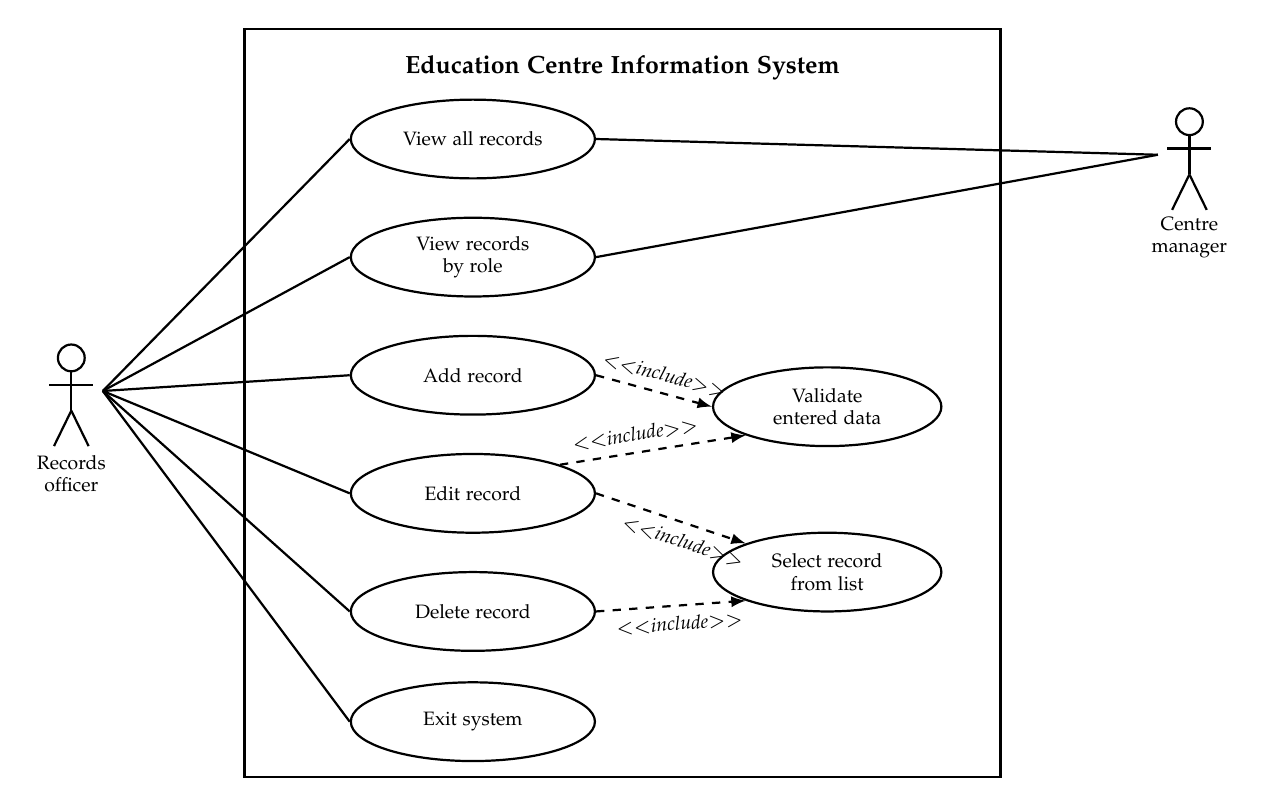
\begin{tikzpicture}[x=1cm,y=1cm]

% --- system boundary ------------------------------------------------------
\draw[thick] (0,0.3) rectangle (9.6,9.8);
\node[font=\small\bfseries] at (4.8,9.3)
     {Education Centre Information System};

% --- the operations offered by the menu -----------------------------------
\node[usecase] (viewall) at (2.9,8.4) {View all records};
\node[usecase] (byrole)  at (2.9,6.9) {View records\\by role};
\node[usecase] (add)     at (2.9,5.4) {Add record};
\node[usecase] (edit)    at (2.9,3.9) {Edit record};
\node[usecase] (delete)  at (2.9,2.4) {Delete record};
\node[usecase] (exit)    at (2.9,1.0) {Exit system};

% --- the two steps shared by more than one operation ----------------------
\node[usecase, minimum width=2.9cm] (validate) at (7.4,5.0) {Validate\\entered data};
\node[usecase, minimum width=2.9cm] (select)   at (7.4,2.9) {Select record\\from list};

% --- actors ---------------------------------------------------------------
\actor{-2.2,5.0}{Records\\officer}{officer}
\actor{12.0,8.0}{Centre\\manager}{manager}

% --- the records officer runs every operation -----------------------------
\draw[assoc] (-1.8,5.2) -- (viewall.west);
\draw[assoc] (-1.8,5.2) -- (byrole.west);
\draw[assoc] (-1.8,5.2) -- (add.west);
\draw[assoc] (-1.8,5.2) -- (edit.west);
\draw[assoc] (-1.8,5.2) -- (delete.west);
\draw[assoc] (-1.8,5.2) -- (exit.west);

% --- the centre manager only reads the records ----------------------------
\draw[assoc] (11.6,8.2) -- (viewall.east);
\draw[assoc] (11.6,8.2) -- (byrole.east);

% --- included use cases ---------------------------------------------------
\draw[depend] (add.east)    -- node[stereo, above, sloped, pos=0.55]
      {\textless\textless include\textgreater\textgreater} (validate.west);
\draw[depend] (edit.north east) -- node[stereo, above, sloped, pos=0.42]
      {\textless\textless include\textgreater\textgreater} (validate.south west);
\draw[depend] (edit.east)   -- node[stereo, below, sloped, pos=0.62]
      {\textless\textless include\textgreater\textgreater} (select.north west);
\draw[depend] (delete.east) -- node[stereo, below, sloped, pos=0.55]
      {\textless\textless include\textgreater\textgreater} (select.south west);

\end{tikzpicture}
\caption{Use case diagram of the Education Centre Desktop Information System.}
\label{fig:usecase}
\end{figure}

\end{document}
